
\begin{enumerate}
The probability distribute of discrete random variable $X$ is tabulated below. There are 5 possible outcome of $X$, i.e. 1, 2, 3, 4 and 5.
\begin{center}
\begin{tabular}{|c||c|c|c|c|c|}
\hline
$x_i$  & 1 & 2 & 3 & 4 & 5  \\\hline
$p(x_i)$ & 0.30 & 0.20 & 0.20 & 0.10 & 0.20 \\
\hline
\end{tabular}
\end{center}

\begin{itemize}
%\item[a.] (1 Mark) Compute the value of $k$.
\item[(a)] (2 Mark) What is the expected value of X?
\item[(b)] (2 Mark) Compute the value of $E(X^2)$
\item[(c)] (2 Mark) Compute the variance of $X$.
\end{itemize}
%-----------------------------------%

\item For the following sample of numbers, calculate the following:\\[0.2cm]
{\bf(a)} Mean. \quad {\bf(b)} Median. \quad {\bf(c)} Standard deviation. \quad {\bf(d)} Inter-quartile range.

\begin{center}
\begin{tabular}{|cccccccccc|}
\hline
&&&&&&&&&\\[-0.4cm]
2 & 4 & 2 & 1 & 5 & 3 & 0 & 4 & 1 & 8 \\
\hline
\end{tabular}
\end{center}



\end{enumerate}


%==================================================================%
\subsection*{Question 1A : Introductory Definitions}





\subsection*{Question 5 : SPSS Output}
%\begin{figure}[h!]
%\centering
%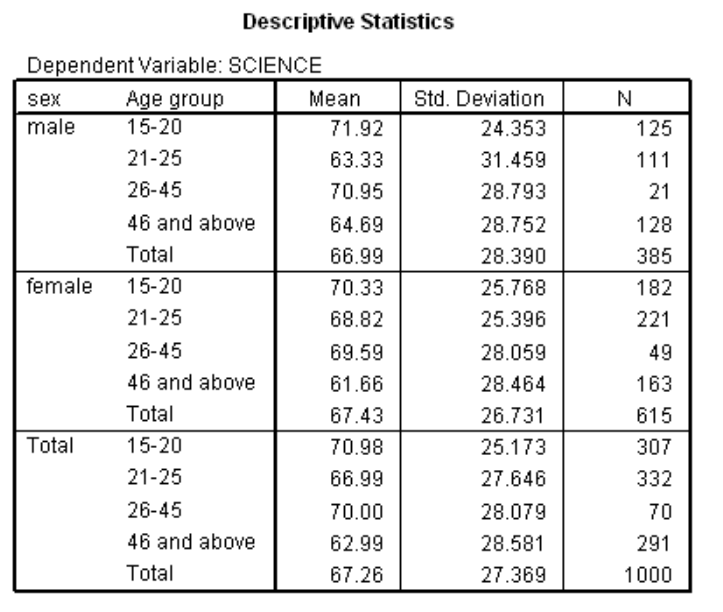
\includegraphics[width=0.65\linewidth]{images/SPSS-Week1}
%\end{figure}
\begin{enumerate}
\item What is the mean Science score for all Males?
\item What it the mean Science score for all Females?
\item What is the mean Science score for everybody in the study?
\item How many respondents are there altogether?
\item How many people are in the 15-20 age group altogether?
\item Which Age group has the highest Score?
%\item What is the smallest age group in the sample?
\end{enumerate}

\section*{Probability Distributions}


\begin{itemize}
\item The discrete uniform distribution
\item The continuous uniform distribution
\item The binomial disribution
\item The poisson distribution
\item The exponential distribution
\item the Normal distribution
\end{itemize}



%\begin{enumerate}
%%--Distributions
%
%
%
%
%\item uniform - The lower and upper bounds are 13cm and 21cm respectively.
%
%\item A computer server breaks down, on average, once every three months.
\begin{itemize}
\item What is the probability that the server breaks down three times in a quarter?
\item What is the probability that a server breaks down exactly five times in one year?
\end{itemize}




%A charity believes that when it puts out an appeal for charitable donations the donations it receives 
%will normally distributed with a mean 50 and 
%
%standard deviation €6, and
%
% it is assumed that donations will be independent of each other.
%
%\begin{itemize} 
%\item Find the probability that the first donation it receives will be less than€40.
%
%\item Compute the probability that it will be between €40and €45.
%\item Compute the value $x$ such that 5\% of donations are more than €$x$.
%\end{itemize}
%

